\documentclass{beamer}
\usepackage{ctex, hyperref}
\usepackage[T1]{fontenc}

% other packages
\usepackage{latexsym,amsmath,xcolor,multicol,booktabs,calligra}
\usepackage{graphicx,pstricks,listings,stackengine}
\usepackage[normalem]{ulem}

\author{userElaina}
\title{Crowdsource}
\institute{School of AI}
\date{2024.06.19}
\usepackage{JilinUniv}

\def\cmd#1{\texttt{\color{red}\footnotesize $\backslash$#1}}
\def\env#1{\texttt{\color{blue}\footnotesize #1}}
\definecolor{deepblue}{rgb}{0,0,0.5}
\definecolor{deepred}{rgb}{0.6,0,0}
\definecolor{deepgreen}{rgb}{0,0.5,0}
\definecolor{halfgray}{gray}{0.55}

\lstset{
    basicstyle=\ttfamily\small,
    keywordstyle=\bfseries\color{deepblue},
    emphstyle=\ttfamily\color{deepred},    % Custom highlighting style
    stringstyle=\color{deepgreen},
    numbers=left,
    numberstyle=\small\color{halfgray},
    rulesepcolor=\color{red!20!green!20!blue!20},
    frame=shadowbox,
}

\begin{document}

\kaishu
\begin{frame}
    \titlepage
    \begin{figure}[htpb]
        \begin{center}
            
\includegraphics[width=0.15\linewidth]{pic/Jilin_University_Logo.eps}
        \end{center}
    \end{figure}
\end{frame}

% \begin{frame}
% \tableofcontents[sectionstyle=show,subsectionstyle=show/shaded/hide,subsubsectionstyle=show/shaded/hide]
% \end{frame}

% \section{Crowdsource}

\begin{frame}{Overview}
    \begin{figure}[c]
        \centering
        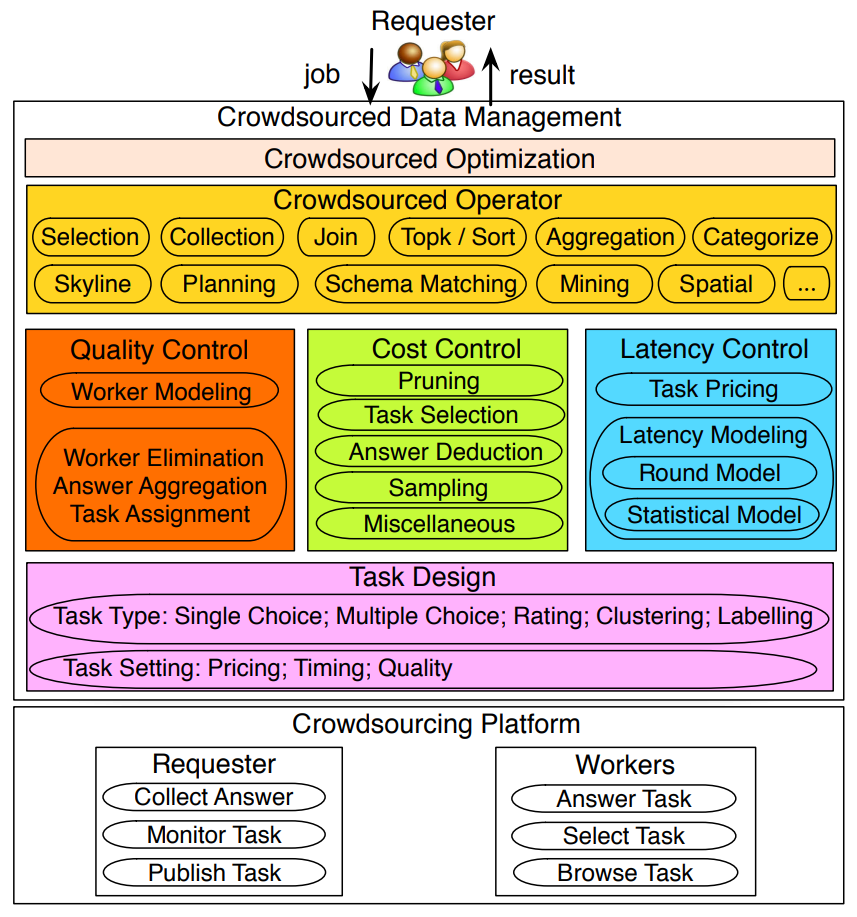
\includegraphics[height=.8\textheight]{pic/1.png}
        \caption{Overview of Crowdsourced Data Management}
    \end{figure}
\end{frame}

\begin{frame}{Quality Control \footnote{Crowdsourced Data Management: A Survey}}
    \begin{itemize}
        \item Worker Modeling: characterize a worker's quality
        \item Improve Quality:
        \begin{itemize}
            \item \sout{Worker Elimination: eliminate the low-quality workers and spammers}
            \item Answer Aggregation: assign a task to multiple workers and aggregate their answers
            \item \sout{Task Assignment: assign tasks to appropriate workers}
        \end{itemize}
    \end{itemize}
\end{frame}

\begin{frame}{Worker Modeling}
    Modeling a Worker:
    \begin{itemize}
        \item Worker Probability: $q \in [0, 1]$
        \begin{itemize}
            \item \begin{gather*}
                q \in [-\infty, +\infty]
            \end{gather*}
            \item \begin{gather*}
                [q_{l, t}, q_{r, t}], \\
                0 \leq q_{l, t} \leq q_{l, t+1} \leq q_{r, t+1} \leq q_{r, t} \leq 1
            \end{gather*}
        \end{itemize}
        \item Confusion Matrix
        \item Bias and Variance: $o \sim \mathcal{N} (t+c, \sigma^2)$
    \end{itemize}
\end{frame}

\begin{frame}{Worker Modeling}
    Modeling a Worker:
    \begin{itemize}
        \item Diverse Skills Across Tasks: $\vec{q} = [q_1, q_2, ..., q_n],$ where $n$ is the number of tasks.
        \item Diverse Skills Across Domains: $\vec{q} = [q_1, q_2, ..., q_K],$ where $K$ is the number of domains (known).
        \begin{itemize}
            \item $K$ latent domains. $K$ is predefined. \footnote{Crowd-Selection Query Processing in Crowdsourcing Databases: A Task-Driven Approach} \footnote{A transfer learning based framework of crowd-selection on twitter}
        \end{itemize}
    \end{itemize}
\end{frame}

\begin{frame}{Worker Modeling}
    Computation of Worker Model Parameters:
    \begin{itemize}
        \item Qualification Test: Golden tasks: tasks with known true answers
        \item Gold-Injected Method: Diff: workers do not know that some golden tasks are injected
        \item EM-Based Methods \footnote{Learning From Crowds} \footnote{Deep Learning From Crowds}
        \item Graph-Based Methods \footnote{Probabilistic graphical models: principles and techniques}
    \end{itemize}
\end{frame}

\begin{frame}{Learning From Crowds}
    Notice:
    \begin{itemize}
        \item $f_w(x) = w^T x$
        \item $\sigma(z) = \frac{1}{1 + e^{−z}}$
        \item $P[y = 1 | x, w] = \sigma(f_w(x)) = \sigma(w^Tx)$
        \item $D = \{x_i, y^1_i, ..., y^R_i\}^N_{i=1}$ training data
        \item $N$ instances
        \item $R$ workers
        \item $\alpha = [\alpha_1, ..., \alpha_R]$ sensitivity
        \item $\beta = [\beta_1, ..., \beta_R]$ specificity
        \item $\theta = \{w, \alpha, \beta\}$ parameters
    \end{itemize}
\end{frame}

\begin{frame}{Learning From Crowds}
    The likelihood function:
    \begin{align*}
        P[D|\theta] &= \Pi^N_{i=1} P[y^1_i, ..., y^R_i | x_i, \theta] \\
        &= \Pi^N_{i=1} (a_ip_i + b_i(1-p_i))
    \end{align*}
    where
    \begin{align*}
        p_i &= \sigma(w^Tx_i) \\
        a_i &= \Pi^R_{j=1} [\alpha_j]^{y_{i,j}} [1-\alpha_j]^{1-y_{i,j}} \\
        b_i &= \Pi^R_{j=1} [\beta_j]^{1-y_{i,j}} [1-\beta_j]^{y_{i,j}}
    \end{align*}
\end{frame}

\begin{frame}{Learning From Crowds}
    E-step:
    \begin{align*}
        \mu_i &\propto P[y^1_i, ..., y^R_i | y_i=1, \theta] P[y_i = 1 | x_i, \theta] \\
        &= \frac{a_ip_i}{a_ip_i + b_i(1-p_i)}
    \end{align*}
    M-step:
    \begin{align*}
        \alpha_j &= \frac{\sum^N_{i=1} \mu_iy_{i,j}}{\sum^N_{i=1} \mu_i} \\
        \beta_j &= \frac{\sum^N_{i=1}(1-\mu_i)(1-y_{i,j})}{\sum^N_{i=1}(1-\mu_i)} \\
    \end{align*}
\end{frame}

\begin{frame}{Learning From Crowds}
    Newton-Raphson:
    \begin{align*}
        w_{t+1} = w_t - \eta H^{-1}g
    \end{align*}
    where:
    \begin{align*}
        g(w) &= \sum^N_{i=1}(\mu_i-\sigma(w^Tx_i)) x_i \\
        H(w) &= -\sum^N_{i=1}\sigma(w^Tx_i)(1-\sigma(w^T x_i)) x_i x_i^T \\
    \end{align*}
\end{frame}

\begin{frame}{Answer Aggregation}
    Voting Strategy:
    \begin{itemize}
        \item Majority Voting
        \item Weighted Majority Voting
        \item Bayesian Voting
    \end{itemize}
\end{frame}

\begin{frame}{Task Types}
    \begin{itemize}
        \item Single Choice
        \item Multiple Choice
        \item Rating
        \item Clustering
        \item Labelling (different: open task)
    \end{itemize}
    to LLM (with Prompt) (Visual or not)
\end{frame}

\end{document}

% Q model para
